\documentclass[a4paper, 10pt]{book}
%1m = 39.4 inch
%大18开 (18.5cm * 23cm)
%\usepackage[left=3.25cm, right=3.25cm, top=2.3cm,bottom=1.4cm]{geometry}
\usepackage{geometry}
\geometry{left=3.75cm,right=3.25cm,top=3cm,bottom=2.5cm}

%% en_preamble包含基本的宏包配置
%%%%%%%%------------------------------------------------------------------------
%%%% 日常所用宏包

%%设置行间距
\usepackage{setspace}

%% 控制项目列表
\usepackage{enumerate}

%% 多栏显示
\usepackage{multicol}

\usepackage[most]{tcolorbox}

%% hyperref宏包,生成可定位点击的超链接,并且会生成pdf书签
\usepackage[%
    pdfstartview=FitH,%
    CJKbookmarks=true,%
    bookmarks=true,%
    bookmarksnumbered=true,%
    bookmarksopen=true,%
    colorlinks=true,%
    citecolor=blue,%
    linkcolor=blue,%
    anchorcolor=green,%
    urlcolor=blue%
]{hyperref}

%% 控制标题
\usepackage{titlesec}

%% 控制表格样式
\usepackage{booktabs}

%% 控制目录
\usepackage{titletoc}

%% 控制字体大小
\usepackage{type1cm}

%% 首行缩进,用\noindent取消某段缩进
\usepackage{indentfirst}

%% 支持彩色文本、底色、文本框等
\usepackage{color,xcolor}

%% AMS LaTeX宏包
\usepackage{amsmath}
\usepackage{amssymb}

\usepackage{multirow}

%% 一些特殊符号
% \usepackage{bbding}

%% 支持引用
% \usepackage{cite}

%% LaTeX一些特殊符号宏包
% \usepackage{latexsym}

%% 数学公式中的黑斜体
% \usepackage{bm}

%% 调整公式字体大小:\mathsmaller, \mathlarger
% \usepackage{relsize}

%% 生成索引
% \makeindex

%%%% 基本插图方法
%% 图形宏包
\usepackage{graphicx}
\usepackage{float}
%% 如果插入的图片没有指定扩展名,那么依次搜索下面的扩展名所对应的文件
\DeclareGraphicsExtensions{.pdf,.eps,.png,.jpg}
%% 让 latex 从 .bb 中读取 Bounding Box 信息
%\DeclareGraphicsRule{.jpg}{eps}{.bb}{}
%\DeclareGraphicsRule{.png}{eps}{.bb}{}
%\DeclareGraphicsRule{.pdf}{eps}{.bb}{}

%% 多个图形并排,参加lnotes.pdf
%\usepackage{subfig}
\usepackage{subfigure}

\usepackage{caption}
\captionsetup{font={sf, scriptsize}, labelfont={bf}, skip=15pt}
\DeclareCaptionLabelSeparator{colon}{~~}

\usepackage[perpage,stable]{footmisc}

\usepackage{longtable}
% \begin{figure}[htbp]               %% 控制插图位置
%   \setlength{\abovecaptionskip}{0pt}
%   \setlength{\belowcaptionskip}{10pt}
                                     %% 控制图形和上下文的距离
%   \centering                       %% 使图形居中显示
%   \includegraphics[width=0.8\textwidth]{CTeXLive2008.jpg}
                                     %% 控制图形显示宽度为0.8\textwidth
%   \caption{CTeXLive2008安装过程} \label{fig:CTeXLive2008}
                                     %% 图形题目和交叉引用标签
% \end{figure}
%%%% 基本插图方法结束

%%%% pgf/tikz绘图宏包设置
\usepackage{pgf,tikz}
\usetikzlibrary{shapes,automata,snakes,backgrounds,arrows}
\usetikzlibrary{mindmap, trees,  calendar}
\usetikzlibrary{positioning}
\usepackage{pgf-umlsd}
%% 可以直接在latex文档中使用graphviz/dot语言,
%% 也可以用dot2tex工具将dot文件转换成tex文件再include进来
%% \usepackage[shell,pgf,outputdir={docgraphs/}]{dot2texi}
%%%% pgf/tikz设置结束


%%%% fancyhdr设置页眉页脚
%% 页眉页脚宏包
\usepackage{fancyhdr}

%% 页眉页脚风格
\pagestyle{fancy}

%%这两行代码是修改\leftmark和\rightmark的经典模式
\renewcommand{\chaptermark}[1]{\markboth{{\hei {第\thechapter{}章}}\hspace 1  #1}{}}
\renewcommand{\sectionmark}[1]{\markright{\thesection{} #1}}

%% 清空当前页眉页脚的默认设置
\fancyhf{}

\renewcommand{\headrulewidth}{0.4pt}
\renewcommand{\footrulewidth}{0.4pt}

%第{\couriernew\thechapter{}}章
%%下面开始修改页眉和页脚
\fancyhead[RE]{\fangsong \leftmark}
\fancyhead[LO]{\fangsong \rightmark}
\fancyhead[RO, LE]{\small \thepage}
\fancypagestyle{plain}{%
  \fancyhead{} % get rid of headers
  \renewcommand{\headrulewidth}{0pt} % and the line.
}

%%定义空白页面
\makeatletter
\def\cleardoublepage{\clearpage\if@twoside \ifodd\c@page\else
  \hbox{}
  \vspace*{\fill}
  \begin{center}
   {\sffamily\large}
   \end{center}
   \vspace{\fill}
   \thispagestyle{empty}
   \newpage
   \if@twocolumn\hbox{}\newpage\fi\fi\fi}
\makeatother

\makeatletter
\def\cleardedicatepage{\clearpage
  \hbox{}
  \vspace*{\fill}
  \begin{center}
   {\sffamily\Large 献给我的女儿刘楚溪}
   \end{center}
   \vspace{\fill}
   \thispagestyle{empty}
   \newpage
   \if@twocolumn\hbox{}\newpage\fi}
\makeatother

%% 有时会出现\headheight too small的warning
\setlength{\headheight}{15pt}

%%%% fancyhdr设置结束

%%设置行间距离
\usepackage{framed}  
%%%% listings宏包设置结束

%%%% 附录设置
\usepackage[title,titletoc,header]{appendix}
%%%% 附录设置结束

%%%% 日常宏包设置结束
%%%%%%%%------------------------------------------------------------------------

%%%%%%%%------------------------------------------------------------------------
%%%% 英文字体设置结束
%% 这里可以加入自己的英文字体设置
%%%%%%%%------------------------------------------------------------------------

%%%%%%%%------------------------------------------------------------------------
%%%% 设置常用字体字号,与MS Word相对应

%% 一号, 1.4倍行距
\newcommand{\yihao}{\fontsize{26pt}{36pt}\selectfont}
%% 二号, 1.25倍行距
\newcommand{\erhao}{\fontsize{22pt}{28pt}\selectfont}
%% 小二, 单倍行距
\newcommand{\xiaoer}{\fontsize{18pt}{18pt}\selectfont}
%% 三号, 1.5倍行距
\newcommand{\sanhao}{\fontsize{16pt}{24pt}\selectfont}
%% 小三, 1.5倍行距
\newcommand{\xiaosan}{\fontsize{15pt}{22pt}\selectfont}
%% 四号, 1.5倍行距
\newcommand{\sihao}{\fontsize{14pt}{21pt}\selectfont}
%% 半四, 1.5倍行距
\newcommand{\bansi}{\fontsize{13pt}{19.5pt}\selectfont}
%% 小四, 1.5倍行距
\newcommand{\xiaosi}{\fontsize{12pt}{18pt}\selectfont}
%% 大五, 单倍行距
\newcommand{\dawu}{\fontsize{11pt}{11pt}\selectfont}
%% 五号, 单倍行距
\newcommand{\wuhao}{\fontsize{10.5pt}{10.5pt}\selectfont}
%%%%%%%%------------------------------------------------------------------------

%%%%%%%%------------------------------------------------------------------------
%%%% 一些个性设置

%% 设定页码方式,包括arabic、roman等方式
%% \pagenumbering{arabic}

%% 有时LaTeX无从断行,产生overfull的错误,这条命令降低LaTeX断行标准
%% \sloppy

%% 设定目录显示深度\tableofcontents
%% \setcounter{tocdepth}{2}
%% 设定\listoftables显示深度
%% \setcounter{lotdepth}{2}
%% 设定\listoffigures显示深度
%% \setcounter{lofdepth}{2}

%% 中文破折号,据说来自清华模板
\newcommand{\pozhehao}{\kern0.3ex\rule[0.8ex]{2em}{0.1ex}\kern0.3ex}

%% 设定itemize环境item的符号
\renewcommand{\labelitemi}{$\bullet$}

%\makeatletter
%\@addtoreset{lstlisting}{section} 
%\makeatother

\usepackage{array,tabularx}
\usepackage{colortbl}

\newenvironment{enum}
{
  \begin{spacing}{1.2}
  % \begin{enumerate}[1.]
  \begin{enumerate}
    \setlength{\itemsep}{0pt} 
    \setlength{\itemindent}{2em}
    %\setlength{\listparindent}{2em}
}{%
  \end{enumerate}
  \end{spacing}
}

\newenvironment{nitemize}
{
  \begin{itemize}
    \setlength{\itemsep}{0pt} 
    \setlength{\itemindent}{2em}
}{%
  \end{itemize}
}


\newcommand{\suggest}[1]{
\tikzstyle{mybox} = [draw=black, very thick,
rectangle, rounded corners, inner sep=9pt, inner ysep=20pt]
\tikzstyle{fancytitle} =[fill=white, text=black, ellipse]
\noindent
\begin{tikzpicture}
\node [mybox] (box){%
\begin{minipage}{\textwidth}
\fangsong
#1
\end{minipage}
};
\node[fancytitle, right=10pt] at (box.north west) {\emph{建议}};
% \node[fancytitle, rounded corners] at (box.east) {$\clubsuit$};
\end{tikzpicture}
}

\newcommand{\notice}[1]{
\tikzstyle{mybox} = [draw=black, very thick,
rectangle, rounded corners, inner sep=9pt, inner ysep=20pt]
\tikzstyle{fancytitle} =[fill=white, text=black]
\noindent
\begin{tikzpicture}
\node [mybox] (box){%
\begin{minipage}{\textwidth}
\fangsong
#1
\end{minipage}
};
\node[fancytitle, right=10pt] at (box.north west) {\emph{注意}};
%\node[fancytitle, rounded corners] at (box.east) {$\clubsuit$};
\end{tikzpicture}
}

\newcommand{\tip}[1]{
\tikzstyle{mybox} = [draw=black, very thick,
rectangle, rounded corners, inner sep=9pt, inner ysep=20pt]
\tikzstyle{fancytitle} =[fill=white, text=black]
\noindent
\begin{tikzpicture}
\node [mybox] (box){%
\begin{minipage}{\textwidth}
\fangsong
#1
\end{minipage}
};
\node[fancytitle, right=10pt] at (box.north west) {\emph{提示}};
%\node[fancytitle, rounded corners] at (box.east) {$\clubsuit$};
\end{tikzpicture}
}

\newcommand\refch[1]{\ascii{第\ref{ch:#1}章(\nameref{ch:#1})}}
\newcommand\refsec[1]{\ascii{\ref{sec:#1}节(\nameref{sec:#1})}}

% \newcommand\eitem[1]{\item {\optima {#1}}}
\newcommand\eitem[1]{\item {\itshape {#1}}}
\newcommand\cpp{\ascii{C\nobreak+\nobreak+}}
\newcommand\clang{\ascii{C}}
\newcommand\tf{\ascii{TensorFlow}}
\newcommand\docker{\ascii{Docker}}
\newcommand\kube{\ascii{Kubernetes}}
\newcommand\apiserver{\ascii{API Server}}
\newcommand\etcd{\ascii{ETCD}}
\newcommand\cm{\ascii{Controller Manager}}
\newcommand\sche{\ascii{Scheduler}}
\newcommand\Pod{\ascii{Pod}}
\newcommand\svc{\ascii{Service}}
\newcommand\ep{\ascii{Endpoint}}
\newcommand\vip{\ascii{ClusterIP}}

\newcommand\quo[1]{“#1”}

\newcommand\percent[1]{\ascii{#1\%}}

\newcommand{\trans}{\emph{事务}}
\newcommand{\act}{\emph{操作}}
\newcommand{\seqact}{\emph{顺序操作}}
\newcommand{\conact}{\emph{并发操作}}
\newcommand{\atomact}{\emph{基本操作}}
\newcommand{\syncact}{\emph{同步操作}}
\newcommand{\asynact}{\emph{异步操作}}
\newcommand{\action}[1]{\emph{\ascii{\itshape\_\_#1}}}
\newcommand{\sigwait}{\action{sig\_wait}}
\newcommand{\sigsync}{\action{sig\_sync}}
\newcommand{\sigreply}{\action{sig\_reply}}
\newcommand{\timerprot}{\action{timer\_prot}}
\newcommand{\unknownevet}{\ascii{UNKNOWN\_EVENT}}
\newcommand{\transdsl}{\ascii{Transaction DSL}}
\newcommand{\oper}[1]{\ascii{Action#1}}
\newcommand{\protproc}{\ascii{prot\_procedure}}

%\newcommand{\code}[1]{\ascii{\small{\texttt{#1}}}}
\newcommand{\code}[1]{\ascii{\footnotesize{\texttt{#1}}}}
\newcommand{\script}[1]{\ascii{\scriptsize{\texttt{#1}}}}


\newcommand{\inlinetitle}[1]{\large{\emph{#1}}}

%\newcommand{\Email}{\begingroup \def\UrlLeft{<}\def\UrlRight{>} \urlstyle{tt}\Url}
%\def\mailto|#1|{\href{mailto:#1}{Email|#1|}}
\newcommand{\contrib}[2]{#1\quad{\small\quad\textit{#2}}\\[1ex]}


\newcommand{\upcite}[1]{\textsuperscript{\cite{#1}}}

% todo list

% 使用方法
% \todobox{
%   \begin{todolist}
%   \item[\done] Frame the problem
%   \item Write solution
%   \item[\wontfix] profit
%   \end{todolist}
% }

\newcommand{\todobox}[1]{
\tikzstyle{mybox} = [draw=black, very thick,
rectangle, rounded corners, inner sep=9pt, inner ysep=20pt]
\tikzstyle{fancytitle} =[fill=white, text=black]
\noindent
\begin{tikzpicture}
\node [mybox] (box){%
\begin{minipage}{\textwidth}
\fangsong
#1
\end{minipage}
};
\node[fancytitle, right=10pt] at (box.north west) {\emph{TODO列表}};
%\node[fancytitle, rounded corners] at (box.east) {$\clubsuit$};
\end{tikzpicture}
}

\newtcolorbox{episode}[1]{enhanced jigsaw,breakable,pad at break*=1mm,colback=red!5!white, colframe=red!75!black,fonttitle=\bfseries, colbacktitle=red!85!black,enhanced, watermark color=white,watermark text=\Roman{tcbbreakpart},center title,title=#1}

\newtcolorbox[auto counter,number within=chapter]{nodiff}[1]{left=0mm,right=0mm,enhanced jigsaw,breakable,pad at break*=1mm,colback=red!5!white,colframe=red!75!black,fonttitle=\footnotesize\bfseries, colbacktitle=red!85!black,enhanced, attach boxed title to top left={yshift=-2mm}, watermark color=white,title=\code{#1}}

\newtcolorbox[auto counter,number within=chapter]{diff}[1]{toggle enlargement=forced,spread inwards=-2cm,spread outwards=-1.5cm,left=0mm,right=0mm,enhanced jigsaw,breakable,pad at break*=1mm,colback=red!5!white,colframe=red!75!black,fonttitle=\footnotesize\bfseries, colbacktitle=red!85!black,enhanced, attach boxed title to top left={yshift=-2mm}, watermark color=white,title=\code{#1},sidebyside,sidebyside align=top,sidebyside gap=2mm}

\newtcolorbox{inlinediff}{opacityframe=0.0,opacityback=0.0,boxrule=0.0mm,left=0mm,right=0mm,sidebyside,sidebyside align=top,sidebyside gap=2mm}

\newtcolorbox[auto counter,number within=chapter]{topdiff}[1]{toggle enlargement=forced,spread inwards=-2cm,spread outwards=-1.5cm,bottomrule=0mm,left=0mm,right=0mm,enhanced jigsaw,breakable,pad at break*=1mm,colback=red!5!white,colframe=red!75!black,fonttitle=\bfseries, colbacktitle=red!85!black,enhanced, attach boxed title to top left={yshift=-2mm}, watermark color=white,title=\code{#1},sidebyside,sidebyside align=top,sidebyside gap=2mm}

\newtcolorbox{mindiff}{toggle enlargement=forced,spread inwards=-2cm,spread outwards=-1.5cm, toprule=0mm,bottomrule=0mm,left=0mm,right=0mm,enhanced jigsaw,breakable,pad at break*=1mm,colback=red!5!white,colframe=red!75!black, colbacktitle=red!85!black,enhanced, attach boxed title to top left={yshift=-2mm}, watermark color=white,sidebyside,sidebyside align=top,sidebyside gap=2mm}

\newtcolorbox{lastdiff}{toggle enlargement=forced,spread inwards=-2cm,spread outwards=-1.5cm,toprule=0mm,left=0mm,right=0mm,enhanced jigsaw,breakable,pad at break*=1mm,colback=red!5!white,colframe=red!75!black, colbacktitle=red!85!black,enhanced, attach boxed title to top left={yshift=-2mm}, watermark color=white,sidebyside,sidebyside align=top,sidebyside gap=2mm}

\newtcolorbox{colortable}[2]{leftright skip=2cm,enhanced,fonttitle=\bfseries,fontupper=\footnotesize\sffamily,
colback=red!5!white,colframe=red!75!black, colbacktitle=red!85!black,center title,tabularx*={\arrayrulewidth0.25mm}{#1},title=#2}

\usepackage{enumitem,amssymb}
\usepackage{pifont}

\newlist{todolist}{itemize}{2}
\setlist[todolist]{label=$\square$}

\newcommand{\cmark}{\ding{51}}%
\newcommand{\xmark}{\ding{55}}%
\newcommand{\done}{\rlap{$\square$}{\raisebox{2pt}{\large\hspace{1pt}\cmark}}%
\hspace{-2.5pt}}
\newcommand{\wontfix}{\rlap{$\square$}{\large\hspace{1pt}\xmark}}


%% 设定正文字体大小
% \renewcommand{\normalsize}{\sihao}

%%%% 个性设置结束
%%%%%%%%------------------------------------------------------------------------




%%%%%%%%------------------------------------------------------------------------
%%%% bibtex设置

%% 设定参考文献显示风格

%%%% bibtex设置结束
%%%%%%%%------------------------------------------------------------------------


%% 如果不写中文的话就不需要引用xecjk_preamble里面的配置
%%%%%%%%------------------------------------------------------------------------
%%%% xeCJK相关宏包

\usepackage{xltxtra,fontspec,xunicode}

%% \CJKsetecglue{\hskip 0.15em plus 0.05em minus 0.05em}
%% slanfont: 允许斜体
%% boldfont: 允许粗体
%% CJKnormalspaces: 仅忽略汉字之间的空白,但保留中英文之间的空白。 
%% CJKchecksingle: 避免单个汉字单独占一行。
\usepackage[slantfont, boldfont]{xeCJK} 
% \usepackage{ctex}

%% 针对中文进行断行
\XeTeXlinebreaklocale "zh"             

%% 给予TeX断行一定自由度
\XeTeXlinebreakskip = 0pt plus 1pt minus 0.1pt

%%%% xeCJK设置结束                                       
%%%%%%%%------------------------------------------------------------------------

%%%%%%%%------------------------------------------------------------------------
%%%% xeCJK字体设置

%% 设置中文标点样式,支持quanjiao、banjiao、kaiming等多种方式
\punctstyle{quanjiao}                                        
                                                     
%% 设置缺省中文字体
\setCJKmainfont[BoldFont={Adobe Heiti Std}, ItalicFont={Adobe Kaiti Std}]{Adobe Song Std}
% \setCJKmainfont[BoldFont={Adobe Heiti Std}, ItalicFont={Adobe Kaiti Std}]{Adobe Song Std}   %  FZBaoSongZ04
%% 设置中文无衬线字体
\setCJKsansfont[BoldFont={Adobe Heiti Std}, ItalicFont={Adobe Kaiti Std}]{Adobe Kaiti Std}  
%% 设置等宽字体
\setCJKmonofont{Adobe Heiti Std}                            
%\setCJKmonofont{Monaco}                            

%% 英文衬线字体
\setmainfont{Lucida Bright}                                  
%% 英文等宽字体
%\setmonofont{Courier}
\setmonofont{Monaco}                             
%\setmonofont{Consolas}                              
%% 英文无衬线字体
\setsansfont{Optima}                                   

%% 定义新字体
\setCJKfamilyfont{song}{Adobe Song Std}                     
\setCJKfamilyfont{kai}{Adobe Kaiti Std}
\setCJKfamilyfont{hei}{Adobe Heiti Std}
\setCJKfamilyfont{fangsong}{Adobe Song Std}
\setCJKfamilyfont{lisu}{LiShu}
\setCJKfamilyfont{youyuan}{Adobe Kaiti Std}

%%自定义英文字体
\newfontfamily\couriernew{Lucida Grande}
\newfontfamily\optima{Optima}
\newfontfamily\lucida{Lucida Bright}

\newcommand{\ascii}[1]{{\optima #1}}
% \newcommand{\ascii}[1]{{\sffamily #1}}
\newcommand{\speak}[1]{{\itshape #1}}
\renewcommand{\emph}[1]{{\hei #1}}

%% 自定义宋体
\newcommand{\song}{\CJKfamily{song}}                       
%% 自定义楷体
\newcommand{\kai}{\CJKfamily{kai}}                         
%% 自定义黑体
\newcommand{\hei}{\CJKfamily{hei}}                         
%% 自定义仿宋体
\newcommand{\fangsong}{\CJKfamily{fangsong}}               
%% 自定义隶书
\newcommand{\lisu}{\CJKfamily{lisu}}                       
%% 自定义幼圆
\newcommand{\youyuan}{\CJKfamily{youyuan}}                 

%%%% xeCJK字体设置结束
%%%%%%%%------------------------------------------------------------------------

%%%%%%%%------------------------------------------------------------------------
%%%% 一些关于中文文档的重定义

%% 数学公式定理的重定义

\newtheorem{example}{例}[section]                                   
\newtheorem{algorithm}{算法}
%% 按section编号
\newtheorem{theorem}{定理}[section]                         
\newtheorem{definition}{定义}
\newtheorem{axiom}{公理}
\newtheorem{property}{性质}
\newtheorem{proposition}{命题}
\newtheorem{lemma}{引理}
\newtheorem{corollary}{推论}
\newtheorem{condition}{条件}
\newtheorem{conclusion}{结论}
\newtheorem{assumption}{假设}

\newtheorem{principle}{原则}[section]
\newtheorem{regulation}{规则}[section]
\newtheorem{advise}{建议}[section]
\newtheorem{concept}{概念}[section]

\usepackage{titlesec}

\renewcommand{\partname}{}
\renewcommand{\thepart}{第\Roman{part}部分}

%% 章节等名称重定义
\renewcommand{\contentsname}{目录}
%\renewcommand{\abstractname}{摘要}
\renewcommand{\indexname}{索引}
\renewcommand{\listfigurename}{插图目录}
\renewcommand{\listtablename}{表格目录}
\renewcommand{\figurename}{图}
\renewcommand{\tablename}{表}
\renewcommand{\appendixname}{附录}
\renewcommand{\appendixpagename}{附录}
\renewcommand{\appendixtocname}{附录}
%\renewcommand\refname{参考文献} 

%%设置内容环境
\newenvironment{content}{%
  \setlength{\parskip}{0.5\baselineskip}
  \begin{spacing}{1.5}
}{%
  \end{spacing}
  \setlength{\parskip}{-0.5\baselineskip}
  \vskip -0.5\baselineskip
}

% 插入小段故事的语法:
% \begin{story}
%   \begin{center}
%     \inlinetitle{分水岭}
%   \end{center}
% \end{story}
\newenvironment{story}
{
  \setlength{\parskip}{0.5\baselineskip}
  \hbox to \textwidth{\hfil\rule{\linewidth}{1.0mm}\hfil}
  \begin{spacing}{1.0}
}{%
  \end{spacing}
  \hbox to \textwidth{\hfil\rule{\linewidth}{1.0mm}\hfil}
  \setlength{\parskip}{-0.5\baselineskip}
  \vskip -0.5\baselineskip
}

%% 设置chapter、section与subsection的格式
%\titleformat{\chapter}[display]{\flushright\yihao}{\thechapter{}}{1em}{\textbf}
\titleformat{\section}[block]{\flushleft\sanhao}{\optima{\thesection}}{1em}{\textbf}
\titleformat{\subsection}{\sihao}{\optima{\thesubsection}}{0.5em}{\textbf}
\titleformat{\subsubsection}{\xiaosi}{\thesubsubsection}{0.5em}{\textbf}

%\titlespacing{\chapter}{0pt}{0pt}{-\baselineskip}
\titlespacing{\section}{0pt}{0pt}{0\baselineskip}
\titlespacing{\subsection}{0pt}{0.5\baselineskip}{0\baselineskip}

%% 设置章格式
\usepackage{quotchap}

\renewcommand\chapterheadstartvskip{
   \vspace*{-5\baselineskip}
}

\renewcommand\chapterheadendvskip{
   \vspace*{0.5\baselineskip}
}

\usepackage{helvet}
\renewcommand\sectfont{\rmfamily\bfseries}

\newcommand\refig[1]{{\itshape \figurename\ascii{\ref{fig:#1}(第\pageref{fig:#1}页)}}}
\newcommand\reftbl[1]{{\itshape \tablename\ascii{\ref{tbl:#1}(第\pageref{tbl:#1}页)}}}

\renewcommand{\footnoterule}{\vspace*{3pt}%
  \hrule width 0.382\textwidth height 0.4pt \vspace*{2.6pt}}

% Remark
\newenvironment{remark}{\par\vskip10pt\footnotesize\itshape % Vertical white space above the remark and smaller font size
\begin{list}{}{
\leftmargin=35pt % Indentation on the left
\rightmargin=25pt}\item\ignorespaces % Indentation on the right
\makebox[-2.5pt]{\begin{tikzpicture}[overlay]
\node[draw=red!60,line width=1pt,circle,fill=red!25,font=\sffamily\bfseries,inner sep=2pt,outer sep=0pt] at (-15pt,0pt){\textcolor{red}{R}};\end{tikzpicture}}
\advance\baselineskip -1pt}{\end{list}\vskip5pt}

%%%% 中文重定义结束
%%%%%%%%------------------------------------------------------------------------


%%%% 设置listings宏包用来粘贴源代码
%% 方便粘贴源代码,部分代码高亮功能
\usepackage{listings}
\usepackage{color}

\DeclareCaptionFont{red}{\color{red}}

%% 所要粘贴代码的编程语言
\lstloadlanguages{{[LaTeX]TeX}, {[ISO]C++}, {Java}, {Ruby}, {Python}, {Scala}}

% Some useful colors...
\definecolor{darkviolet}{rgb}{0.5,0,0.4}
\definecolor{darkgreen}{rgb}{0,0.4,0.2} 
\definecolor{darkblue}{rgb}{0.1,0.1,0.9}
\definecolor{darkgrey}{rgb}{0.5,0.5,0.5}
\definecolor{lightblue}{rgb}{0.4,0.4,1}

\definecolor{stringColor}{rgb}{0.16,0.00,1.00}
\definecolor{annotationColor}{rgb}{0.39,0.39,0.39}
\definecolor{keywordColor}{rgb}{0.50,0.00,0.33}
\definecolor{commentColor}{rgb}{0.25,0.50,0.37}
\definecolor{javadocColor}{rgb}{0.25,0.37,0.75}
\definecolor{jTagColor}{rgb}{0.50,0.62,0.75}
\definecolor{eTagColor}{rgb}{0.50,0.62,0.75}
\definecolor{lineNumberColor}{rgb}{0.47,0.47,0.47}

% Example:
% \lstdefinestyle{SQL}{
%     language={SQL},basicstyle=\ttfamily, 
%     moredelim=**[is][\btHL]{`}{`},
%     moredelim=**[is][{\btHL[fill=orange!30,draw=red,dashed,thin]}]{@}{@},
% }
% 
% A listing with {\btHL highlighting of all \textbf{important} elements} looks as follows:
% 
% \begin{lstlisting}[style=SQL]
% SELECT name, password `FROM` users @WHERE@ name=@UNION SELECT@
% \end{lstlisting}
%
\makeatletter
\newenvironment{btHighlight}[1][]
{\begingroup\tikzset{bt@Highlight@par/.style={#1}}\begin{lrbox}{\@tempboxa}}
{\end{lrbox}\bt@HL@box[bt@Highlight@par]{\@tempboxa}\endgroup}

\newcommand\btHL[1][]{%
  \begin{btHighlight}[#1]\bgroup\aftergroup\bt@HL@endenv%
}
\def\bt@HL@endenv{%
  \end{btHighlight}%   
  \egroup
}
\newcommand{\bt@HL@box}[2][]{%
  \tikz[#1]{%
    \pgfpathrectangle{\pgfpoint{1pt}{0pt}}{\pgfpoint{\wd #2}{\ht #2}}%
    \pgfusepath{use as bounding box}%
    \node[anchor=base west, fill=green!30,outer sep=0pt,inner xsep=0pt, inner ysep=0pt, rounded corners=0.5pt, minimum height=\ht\strutbox+1.1pt,#1]{\raisebox{1.1pt}{\strut}\strut\usebox{#2}};
  }%
}
\makeatother

%% 设置listings宏包的一些全局样式
%% 参考http://hi.baidu.com/shawpinlee/blog/item/9ec431cbae28e41cbe09e6e4.html
\lstset{
numberbychapter=true,
breakatwhitespace=true,
showstringspaces=false,              %% 设定是否显示代码之间的空格符号
basicstyle=\scriptsize\ttfamily,           %% 设定字体大小\tiny, \scriptsize, \footnotesize, \small, \Large等等
keywordstyle=\color{keywordColor}\bfseries,
commentstyle=\color{red!50!green!50!blue!50},      
stringstyle=\color{stringColor},  
escapechar=`,                        %% 中文逃逸字符,用于中英混排
xleftmargin=1.5em,xrightmargin=0em, aboveskip=1.0em,
breaklines,                          %% 这条命令可以让LaTeX自动将长的代码行换行排版
extendedchars=false,                 %% 这一条命令可以解决代码跨页时,章节标题,页眉等汉字不显示的问题
frameround=fttt,
captionpos=top,
belowcaptionskip=1em
}

\lstdefinestyle{numbers}{
   numbers=left,
   numberstyle=\tiny\color{lineNumberColor}\lstfontfamily,
   stepnumber=1,
   numbersep=1em,
}

\lstdefinestyle{C++}{
   language=C++,
   texcl=true,
   prebreak=\textbackslash,
   breakindent=1em,
   emphstyle=\bfseries,
   keywordstyle=\color{keywordColor}\bfseries, %% 关键字高亮
   stringstyle=\color{stringColor},  
   morekeywords={alignas, alignof, char16_t, char32_t, constexpr, decltype, noexcept, nullptr, static_assert, thread_local, override, final},
   moredelim=**[is][\btHL]{@}{@},
   %style=numbers,
   %frame=leftline,                     %% 给代码加框
   %framerule=2pt,
   %rulesep=5pt
}

\lstnewenvironment{minicpp}[1][]
  {\setstretch{1}
  \lstset{style=C++, xleftmargin=0.0em, #1}}
  {}

\lstnewenvironment{c++}[1][]
  {\setstretch{1}
  \lstset{style=C++, #1}}
  {}


%\captionsetup[lstlisting]{textfont=red}
%{labelfont=bf, singlelinecheck=off, labelsep=space, textfont=red}

\lstdefinestyle{Java}{
   language=Java,
   texcl=true,
   prebreak=\textbackslash,
   breakindent=1em,
   keywordstyle=\bfseries, %% 关键字高亮
   morekeywords={}
   style=numbers,
   %frame=leftline,                     %% 给代码加框
   %framerule=2pt,
   %rulesep=5pt
}

\lstnewenvironment{java}[1][]
  {\setstretch{1}
  \lstset{style=Java, #1}}
  {}

\lstdefinestyle{Ruby}{
   language=Java,
   texcl=true,
   prebreak=\textbackslash,
   breakindent=1em,
   keywordstyle=\bfseries, %% 关键字高亮
   morekeywords={}
   style=numbers,
   %frame=leftline,                     %% 给代码加框
   %framerule=2pt,
   %rulesep=5pt
}

\lstnewenvironment{ruby}[1][]
  {\setstretch{1}
  \lstset{style=Ruby, #1}}
  {}

\lstdefinestyle{Python}{
   language=Python,
   texcl=true,
   prebreak=\textbackslash,
   breakindent=1em,
   emphstyle=\bfseries,
   keywordstyle=\color{keywordColor}\bfseries, %% 关键字高亮
   stringstyle=\color{stringColor},  
   morekeywords={with, as},
   moredelim=**[is][\btHL]{@}{@},
   %frame=leftline,                     %% 给代码加框
   %framerule=2pt,
   %rulesep=5pt
}

\lstnewenvironment{python}[1][]
  {\setstretch{1}
  \lstset{style=Python, #1}}
  {}

\lstdefinestyle{Scala}{
   language=Scala,
   texcl=true,
   prebreak=\textbackslash,
   breakindent=1em,
   keywordstyle=\bfseries, %% 关键字高亮
   morekeywords={}
   style=numbers,
   %frame=leftline,                     %% 给代码加框
   %framerule=2pt,
   %rulesep=5pt
}

\lstnewenvironment{scala}[1][]
  {\setstretch{1}
  \lstset{style=Scala, #1}}
  {}  

\renewcommand{\lstlistingname}{示例代码}
\renewcommand\thefigure{\thechapter-\arabic{figure}}

\newcommand\refcode[1]{{\itshape \lstlistingname\ascii{\ref{code:#1}(第\pageref{code:#1}页)}}}



% \usepackage[
%   placement=center,
%   angle=45,
%   scale=20,
%   color=black!40,
%   %hshift=60,
%   %vshift=-5
% ]{background}

% \backgroundsetup{contents={样章}}
% \backgroundsetup{contents={\includegraphics[width=0.2\textwidth]{figures/cock.jpg}}}

\newcommand{\myclearpage}{\clearpage{\pagestyle{empty}\cleardoublepage}}
\newcommand{\mydedicate}{\clearpage{\pagestyle{empty}\cleardedicatepage}}

\begin{document}

\frontmatter
\pagestyle{empty}

\def\titlename{Bazel Build}
\def\subtitle{Build and test software of any size, quickly and reliably}
\def\authors{刘光聪\ 著}
% \def\orgnization{\ascii{}}


\newlength{\centeroffset}
\setlength{\centeroffset}{-0.5\oddsidemargin}
\addtolength{\centeroffset}{0.5\evensidemargin}
\thispagestyle{empty}

% \begin{tikzpicture}
%   \path[mindmap,concept color=black,text=white]
%     node[concept] {\ascii{Programming}}
%     [clockwise from=0]
%     child[concept color=green!50!black] {
%       node[concept] {\ascii{XP}}
%       [clockwise from=90]
%       child { node[concept] {\ascii{Simple Design}} }
%       child { node[concept] {\ascii{TDD}} }
%       child { node[concept] {\ascii{Refactoring}} }
%       child { node[concept] {\ascii{Pair Programming}} }
%     }
%     child[concept color=blue] {
%       node[concept] {\ascii{Oriented-Object}}
%       [clockwise from=-30]
%       child { node[concept] {\ascii{C++}} }
%       child { node[concept] {\ascii{Java}} }
%     }
%     child[concept color=red]
%     { node[concept] {\ascii{Evolutionary Design}} }
%     child[concept color=orange]
%     { node[concept] {\ascii{Clean Code}} };
%  \end{tikzpicture}

%title and subtitle
\vspace*{\stretch{1}}
\noindent\hspace*{\centeroffset}\makebox[0pt][l]{\begin{minipage}{\textwidth}
\flushright
{\Huge \hei \bfseries \titlename}
\noindent\rule[-1ex]{\textwidth}{5pt}\\[2.5ex]
\hfill\emph{\subtitle}
\end{minipage}}

%author
\vspace{\stretch{2}}
\noindent\hspace*{\centeroffset}\makebox[0pt][l]{\begin{minipage}{\textwidth}
\center
{\bfseries \authors} \\[1.5ex]
% {\bfseries \orgnization}
\end{minipage}}

\vspace{\stretch{1}}

\pagebreak

\myclearpage

\mydedicate

\tableofcontents
\myclearpage

\def\thelstlisting{\thechapter-\arabic{lstlisting}}
%% 中文习惯是设定首行缩进为2em。
%% 注意此设置一定要在document环境之中,这可能与\setlength作用范围相关
\setlength{\parindent}{2em}

%%%%%%%%%%%%%%%%%%%%%%
%%开始正文,页面计数从正文开始
\mainmatter
\setcounter{page}{1}
\pagestyle{fancy}

\begin{savequote}[45mm]
\ascii{Any fool can write code that a computer can understand. Good programmers write code that humans can understand.}
\qauthor{\ascii{- Martin Flower}}
\end{savequote}

\chapter{破冰之旅} 
\label{ch:bazel-tour}

\section{安装}

\begin{content}

本例以\ascii{Ubuntu 18.04}为例,讲述\ascii{Bazel}的安装方式。

\subsection{二进制安装}

首先,安装\ascii{Bazel}所依赖包。

\begin{nodiff}{安装依赖}
 \begin{python}
$ sudo apt-get install pkg-config zip g++ zlib1g-dev unzip python
 \end{python}
\end{nodiff}

从\ascii{Github}上下载\ascii{Bazel}最新的版本,此处以版本\ascii{0.23.0}为例。

\begin{nodiff}{下载安装包}
 \begin{python}
$ bazel_version=0.23.0
$ bazel_binary=https://github.com/bazelbuild/bazel/releases/download/
$ bazel_binary+=$bazel_version/bazel-$bazel_version-installer-linux-x86_64.sh
$ wget -c $bazel_binary
 \end{python}
\end{nodiff}

修改脚本的权限,运行脚本启动安装过程。使用\ascii{--user}选项,\ascii{Bazel}将安装到\ascii{~/home/bin}目录。

\begin{nodiff}{安装Bazel}
 \begin{python}
$ chmod +x bazel-$bazel_version-installer-linux-x86_64.sh
$ ./bazel-$bazel_version-installer-linux-x86_64.sh --user
 \end{python}
\end{nodiff}

添加\ascii{~/home/bin}目录至环境变量\ascii{PATH}之中。

\begin{nodiff}{添加PATH}
 \begin{python}
$ echo 'export PATH=$PATH:$HOME/bin' >> ~/.bashrc
$ source ~/.bashrc
 \end{python}
\end{nodiff}

最后,通过执行如下命令验证安装是否成功。

\begin{nodiff}{验证}
 \begin{python}
$ bazel version
 \end{python}
\end{nodiff}

\subsection{APT安装}

在\ascii{Ubutu}中,也可以使用\ascii{apt}安装\ascii{Bazel}。因为\ascii}{Bazel}主要使用\ascii{Java}实现,因此需要实现安装\ascii{JVM}。

\begin{nodiff}{安装依赖}
 \begin{python}
$ sudo apt-get install openjdk-8-jdk
 \end{python}
\end{nodiff}

在系统添加\ascii{Bazel}的软件源。

\begin{nodiff}{Bazel源}
 \begin{python}
$ cat <<EOF | sudo tee /etc/apt/sources.list.d/bazel.list
deb [arch=amd64] http://storage.googleapis.com/bazel-apt stable jdk1.8
EOF
$ curl https://bazel.build/bazel-release.pub.gpg | sudo apt-key add -
 \end{python}
\end{nodiff}

执行如下命令,安装\ascii{Bazel}。

\begin{nodiff}{安装Bazel}
 \begin{python}
$ sudo apt-get update
$ sudo apt-get install bazel
 \end{python}
\end{nodiff}

\end{content}

\section{入门}

\begin{content}

\subsection{C++工程}

新建一个\ascii{C++}工程,物理组织如\refig{bazel-tour-hello-world-tree}所示。它包括\ascii{lib}和\ascii{main}两个包。\ascii{WORKSPACE}为空文件,表示该项目不依赖于第三方库,仅依赖标准库。

\begin{figure}[H]
\centering
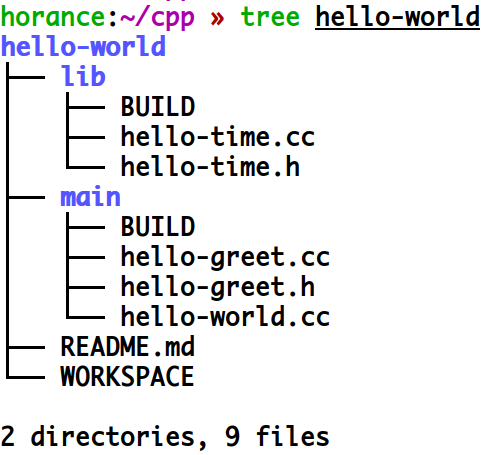
\includegraphics[width=0.5\textwidth]{figures/bazel-tour-hello-world-tree.png}
\caption{工程组织} 
 \label{fig:bazel-tour-hello-world-tree}
\end{figure}

\subsubsection{lib包}

在\ascii{lib}包中,包含\ascii{hello-time.h, hello-time.cc}两个源文件。

\begin{nodiff}{lib/hello-time.h}
 \begin{c++}
#ifndef LIB_HELLO_TIME_H_      
#define LIB_HELLO_TIME_H_

void print_localtime();

#endif
 \end{c++}
\end{nodiff}

\begin{nodiff}{lib/hello-time.cc}
 \begin{c++}
#include "lib/hello-time.h"
#include <ctime>         
#include <iostream>

void print_localtime() {
  std::time_t result = std::time(nullptr);
  std::cout << std::asctime(std::localtime(&result));
}
 \end{c++}
\end{nodiff}

在规则\ascii{//lib:hello-time}定义之中,声明了\ascii{visibility}属性,\ascii{//main:\_\_pkg\_\_}表示该规则对\ascii{main}包可见。

\begin{nodiff}{lib/BUILD}
 \begin{python}
cc_library(
    name = "hello-time", 
    srcs = ["hello-time.cc"], 
    hdrs = ["hello-time.h"],  
    visibility = ["//main:__pkg__"],
)
 \end{python}
\end{nodiff}

\subsubsection{main包}

在\ascii{main}包中,定义了一个规则\ascii{//main:hello-greet},它实现了\ascii{get\_greet}函数。

\begin{nodiff}{main/hello-greet.h}
 \begin{c++}
#ifndef MAIN_HELLO_GREET_H_
#define MAIN_HELLO_GREET_H_

#include <string>

std::string get_greet(const std::string &thing);
      
#endif
 \end{c++}
\end{nodiff}

\begin{nodiff}{main/hello-greet.cc}
 \begin{c++}
#include "main/hello-greet.h"             
#include <string>

std::string get_greet(const std::string& who) {
  return "Hello " + who;
}
 \end{c++}
\end{nodiff}

在\ascii{main}包中,还定义了另一个规则\ascii{//main:hello-world},它实现了\ascii{main}函数。

\begin{nodiff}{main/main.cc}
 \begin{c++}
#include "lib/hello-time.h"
#include "main/hello-greet.h"
#include <iostream>

int main(int argc, char** argv) {
  std::cout << get_greet("world") << std::endl;
  print_localtime();
  return 0;
}
 \end{c++}
\end{nodiff}

重点关注一下规则\ascii{//main:hello-world}的\ascii{deps}属性,因为\ascii{//main:hello-world}和\ascii{//main:hello-greet}在同一个包中,可简写为\ascii{:hello-greet};但是,\ascii{//main:hello-world}和\ascii{//main:hello-time}不在同一个包中,因此需要完整的路径。


\begin{nodiff}{main/BUILD}
 \begin{python}
cc_library(            
    name = "hello-greet",
    srcs = ["hello-greet.cc"],
    hdrs = ["hello-greet.h"], 
) 

cc_binary(
    name = "hello-world",
    srcs = ["hello-world.cc"],
    deps = [             
        ":hello-greet",
        "//lib:hello-time",       
    ],
)
 \end{python}
\end{nodiff}

执行如下命令,构建目标\ascii{//main:hello-world}。

\begin{nodiff}{构建}
 \begin{python}
$ bazel build //main:hello-world
 \end{python}
\end{nodiff}

构建成功后,生成可执行程序\ascii{bazel-bin/main/hello-world}。

\begin{nodiff}{执行}
 \begin{python}
$ bazel-bin/main/hello-world
Hello world
Wed Feb 27 10:49:05 2019
 \end{python}
\end{nodiff}

\subsection{解析依赖}

执行如下命令,可以得到以\ascii{//main:hello-world}为根节点的\ascii{DAG}图,如\refig{bazel-tour-hello-world-deps}所示。

\begin{nodiff}{构建图}
 \begin{python}
$ xdot <(bazel query --nohost_deps --noimplicit_deps 'deps(//main:hello-world)' --output graph)
 \end{python}
\end{nodiff}

\begin{figure}[H]
\centering
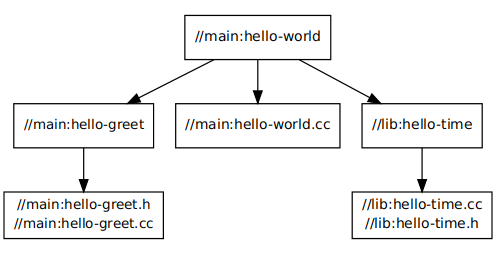
\includegraphics[width=0.8\textwidth]{figures/bazel-tour-hello-world-deps.png}
\caption{依赖图: //main:hello_world} 
 \label{fig:bazel-tour-hello-world-deps}
\end{figure}

\end{content}

\begin{savequote}[45mm]
\ascii{Any fool can write code that a computer can understand. Good programmers write code that humans can understand.}
\qauthor{\ascii{- Martin Flower}}
\end{savequote}

\chapter{原理与概念} 
\label{ch:bazel-concept}

\section{基本概念}

\begin{content}

\subsection{领域模型}

\ascii{Bazel}的核心领域模型非常简单,如\refig{bazel-domain-model}所示。\ascii{Workspace}包含零个或多个\ascii{Package},每个\ascii{Package}包括零个或多个\ascii{Target},\ascii{Target}包括\ascii{File, Rule, PackageGroup}。
 
\begin{figure}[H]
\centering
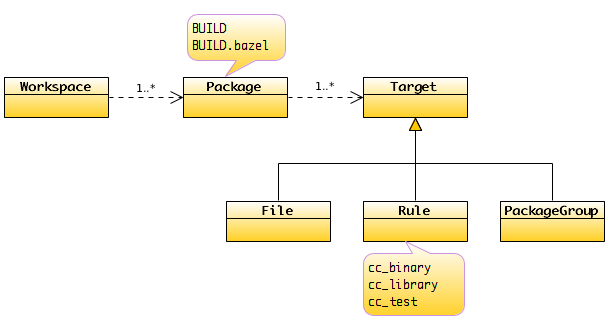
\includegraphics[width=0.9\textwidth]{figures/bazel-domain-model.png}
\caption{领域模型}
 \label{fig:bazel-domain-model}
\end{figure}

\subsection{工作区(Workspace)}

一般地,在项目的\emph{根目录}创建一个\ascii{WORKSPACE}文件,\ascii{Bazel}据此在构建过程中创建一个\emph{工作区}(\ascii{Workspace}),用于标识该项目的起始位置。在工作区内,项目所包含的所有文件,包括待构建的源文件、构建过程中自动生成的文件,及其所有外部依赖都归属于该\emph{工作区}。其中,\ascii{WORKSPACE}文件用于声明本项目的外部依赖;如果项目不存在外部依赖,\ascii{WORKSPACE}的内容可为空。

\subsubsection{隔离环境}

工作区为项目构建提供了一个安全的隔离环境。例如,本地存在两个待构建的\cpp{}项目\ascii{A}和\ascii{B},它们都依赖于第三方\cpp{}库\ascii{D}。不幸的是,它们分别依赖了不同的版本实现\ascii{v1}和\ascii{v2}。如\refig{bazel-concept-conflict}所示,问题变得非常棘手,系统目录\ascii{/usr/local/include, /usr/local/lib}应该放\ascii{D}的哪个版本呢?

\begin{figure}[H]
\centering
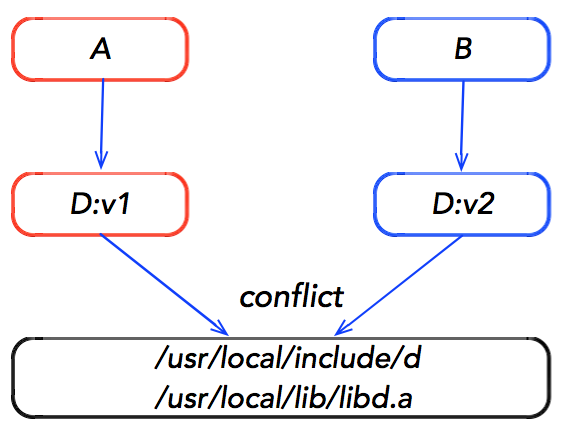
\includegraphics[width=0.5\textwidth]{figures/bazel-concept-conflict.png}
\caption{工作区:隔离构建环境}
 \label{fig:bazel-concept-conflict}
\end{figure}


归功于\ascii{Bazel}良好的隔离性,每个项目的工作区都是独立的,它们将所有依赖控制在各自的工作区,避免了第三方库的名字和版本冲突。如\refig{bazel-concept-workspace}所示。

\begin{figure}[H]
\centering
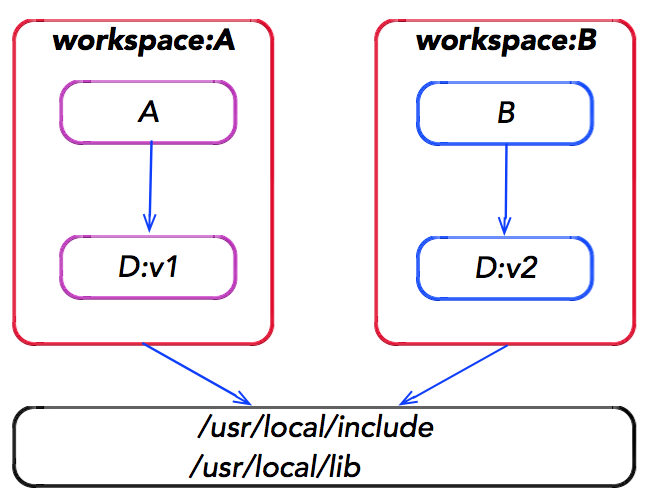
\includegraphics[width=0.5\textwidth]{figures/bazel-concept-workspace.png}
\caption{工作区:隔离构建环境}
 \label{fig:bazel-concept-workspace}
\end{figure}

\subsubsection{惯例优于配置}

按照\ascii{Bazel}的惯例,在项目根目录同时创建一个与项目名称同名的文件夹,以此定义项目命名空间的起始位置。如\refig{bazel-concept-polyflow}所示,项目名称为\ascii{polyflow},在根目录中创建文件\ascii{WORKSPACE},及其同名的子目录\ascii{polyflow};然后在子目录\ascii{polyflow}中,根据系统架构将其分解为两个基本的模块\ascii{core, util}。

\begin{figure}[H]
\centering
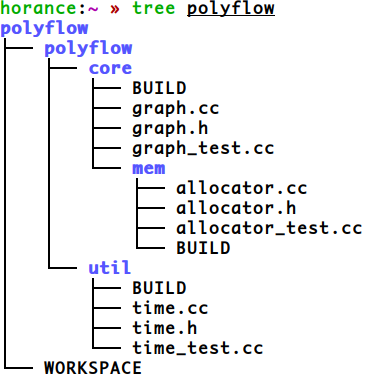
\includegraphics[width=0.6\textwidth]{figures/bazel-concept-polyflow.png}
\caption{Bazel项目组织}
 \label{fig:bazel-concept-polyflow}
\end{figure}

\subsection{包(Package)}

含有\ascii{BUILD}或\ascii{BUILD.bazel}文件的目录,\ascii{Bazel}在构建时将其标识为\emph{包}(\ascii{Package})。如果一个目录不包含\ascii{BUILD}或\ascii{BUILD.bazel}文件,则它只是一个纯粹的目录,隶属于最近的父包(\ascii{BUILD}或\ascii{BUILD.bazel}文件)。

\subsubsection{包名}

包名始于\ascii{WORKSPACE}所在的目录,由路径名组成。例如\ascii{app/core, app/core/mem}\footnote{注意,\ascii{Unix}路径名\ascii{./app/core}与包名\ascii{app/core}不等价,它们之间存在微妙的差异。}。特殊地(常见于遗留系统中),如果\ascii{BUILD}文件与\ascii{WORKSPACE}都在根目录中,此时包名为空,而不是一个点号\footnote{在\ascii{Unix}中,点号表示当前目录。},如\refig{bazel-concept-nil-package}所示。

\begin{figure}[H]
\centering
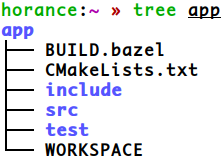
\includegraphics[width=0.35\textwidth]{figures/bazel-concept-nil-package.png}
\caption{包名为空}
 \label{fig:bazel-concept-nil-package}
\end{figure}

\subsubsection{子包}

在一个包中,递归地包含该目录下的所有文件。但是,如果某个子目录自身包含\ascii{BUILD}文件,则独立成为一个子包,并不隶属于上一级的父包。也就是说,子包独立于父包,父包不包括子包。

如\refig{bazel-concept-subpackage}所示,包\ascii{app/core}不包括包\ascii{app/core/mem},它们相互独立。但是,习惯依然称\ascii{app/core/mem}为\ascii{app/core}的子包。

\begin{figure}[H]
\centering
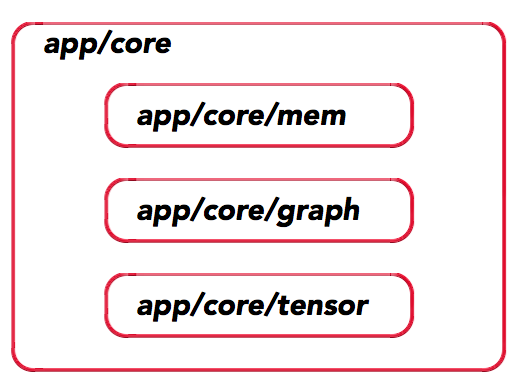
\includegraphics[width=0.4\textwidth]{figures/bazel-concept-subpackage.png}
\caption{子包}
 \label{fig:bazel-concept-subpackage}
\end{figure}



\subsection{目标(Target)}

在一个包(\ascii{Package})中,可以包含零个或多个\emph{目标}(\ascii{Target})。一般地,目标包括\emph{文件}(\ascii{File}),\emph{规则}(\ascii{Rule}),\emph{包集合}(\ascii{Package Group})三种基本类型。

\subsubsection{文件}

文件包括\emph{源文件}和\emph{派生文件}两种基本类型。例如,程序员实现的\cpp{}头文件和实现文件则称为源文件,而由\ascii{protoc}自动生成的\cpp{}头文件和实现文件则称为派生文件。

\subsubsection{规则}

在\ascii{BUILD}文件中,可以定义零个或多个\emph{规则}(\ascii{Rule})。规则由输入、输出、动作三元祖构成。因为\ascii{Bazel}使用声明式的表达方式,规则的动作往往是隐式的。例如,使用规则\ascii{cc\_library}时,无需显式地实现\ascii{g++ a.cc -o a.o}。

规则输入的文件,可能是源文件,也可以是其他规则生成的派生文件,常通过\ascii{srcs, hdrs}等属性表示。但是,规则输出的文件,必然是派生文件。此外,规则输出的派生文件,必然与该规则属于同一个包;但是,规则输入的源文件可以来自于其他包。

规则的输入也可以是规则,常通过\ascii{deps}属性表示。通过规则之间的依赖关系,构建了运行时的\ascii{DAG}图。一般地,依赖关系具有多种表现形式,而且与编程语言极其相关。例如,在编译时,\ascii{A}依赖于\ascii{B}的头文件;在链接时,\ascii{A}依赖于\ascii{B}的符号;在运行时,\ascii{A}依赖于\ascii{B}的数据。

\subsubsection{包集合}

包集合较为特殊,它标识一组包。它由\ascii{package\_group}定义。使用包集合,可以很方便地将某一个规则的可见性一并赋予给该包集合,使得该集合所包含的包都可以访问该规则。

\subsection{标签(Label)}

每个\emph{目标}都存在一个全局的名称,称为标签(\ascii{Label}),由如下几个部分组成:

\begin{nodiff}{标签}
 \begin{c++}
label = "@domain//package_name:target_name"
 \end{c++}
\end{nodiff}

其中,\ascii{@domain}, \ascii{//package\_name}, 冒号,\ascii{target\_name}在一些特殊场景下都可省略。例如,在本工作区内,完全可略去\ascii{@domain};但是,如果引用外部依赖的标签,\ascii{@domain}则是必须的。而在同一个包内,也可完全略去\ascii{//package\_name},甚至略去冒号;按照惯例,规则保留冒号,文件略去冒号。

例如,在\ascii{cub/base/BUILD}中定义了一个\ascii{placement}的基础类库,基本覆盖了所有形态的标签格式。

\begin{nodiff}{标签样例://cub/base/BUILD}
 \begin{python}
package(
    default_visibility = [    
        "//visibility:public",    
    ],
)

cc_library(
    name = "placement",
    hdrs = ["placement.h"],
)

cc_test(
    name = "placement_test",
    srcs = ["placement_test.cc"],
    deps = [ 
        ":placement",
        "//cub/algo:loop",
        "//cub/dci",      
        "@xunit_cut//:cut",
        "@xunit_cut//:cut_main",
    ],  
)
 \end{python}
\end{nodiff}

\subsubsection{文件标签}

在规则\ascii{placement\_test}的\ascii{srcs}属性定义中,标签\ascii{placement\_test.cc}略去了域名和包名,及其可选的冒号。也就是说,在\ascii{//cub/base/BUILD}中,如下标签是等价的。

\begin{nodiff}{//cub/base/BUILD}
 \begin{python}
//cub/base:placement_test.cc
:placement_test.cc # 推荐
placement_test.cc
 \end{python}
\end{nodiff}

\subsubsection{规则标签}

而在规则\ascii{placement\_test}的\ascii{deps}属性定义中,标签\ascii{:placement}略去了域名和包名,但保留了冒号,用于显式地标识它是一个规则。也就是说,在\ascii{//cub/base/BUILD}中,如下标签是等价的。

\begin{nodiff}{//cub/base/BUILD}
 \begin{python}
//cub/base:placement
:placement  # 推荐
placement
 \end{python}
\end{nodiff}

但是,标签\ascii{//cub/algo:loop}来自于另一个包\ascii{cub/algo},所以需要显式地给出全路径。

\subsubsection{同名标签}

特殊地,标签\ascii{//cub/dci}等价于\ascii{//cub/dci:dci}。也就是说,当\ascii{target\_name}等于其目录名,则常常略去\ascii{target\_name}。其中,标签\ascii{//cub/dci:dci}定义如下。

\begin{nodiff}{//cub/dci/BUILD}
 \begin{python}
package(
    default_visibility = [    
        "//visibility:public",    
    ],
)

cc_library(
    name = "dci",
    hdrs = ["role.h"],
)
 \end{python}
\end{nodiff}

注意,标签\ascii{//cub/dci}切忌不可略去\ascii{//},标签名以\ascii{//}开头,而\ascii{cub/dci}仅仅为包名。在同一个\ascii{//cub/dci/BUILD}文件中,如下标签都是等价的。

\begin{nodiff}{//cub/dci/BUILD}
 \begin{python}
//cub/dci:dci
//cub/dci
:dci
dci
 \end{python}
\end{nodiff}

\subsubsection{外部标签}

标签\ascii{@xunit\_cut//:cut}来自于第三方库\ascii{xunit\_cut},因此需要显式地加上域名。外部依赖的名称定义于\ascii{WORKSPACE}之中。按照惯例,域名推荐使用\ascii{DNS}名称,例如\ascii{github\_horanceliu\_cut},将极大降低名字冲突的概率。

\begin{nodiff}{WORKSPACE}
 \begin{python}
http_archive(
    name = "xunit_cut",
    sha256 = "f7c2c339a5ab06dc1d16cb03b157a96e6c591f9833f5c072f56af4a8f8013b53",
    strip_prefix = "cut-master",
    urls = [
        "https://github.com/horance-liu/cut/archive/master.tar.gz",
    ],
)
 \end{python}
\end{nodiff}

其中,\ascii{sha256}的值可以通过执行如下命令得到。

\begin{nodiff}{计算SHA256值}
 \begin{python}
$ curl -L https://github.com/horance-liu/cut/archive/master.tar.gz | sha256sum
 \end{python}
\end{nodiff}

\ascii{Cub}依赖于第三方库\ascii{Cut}的关系,如\refig{bazel-concept-cub-deps-cut}所示。

\begin{figure}
\centering
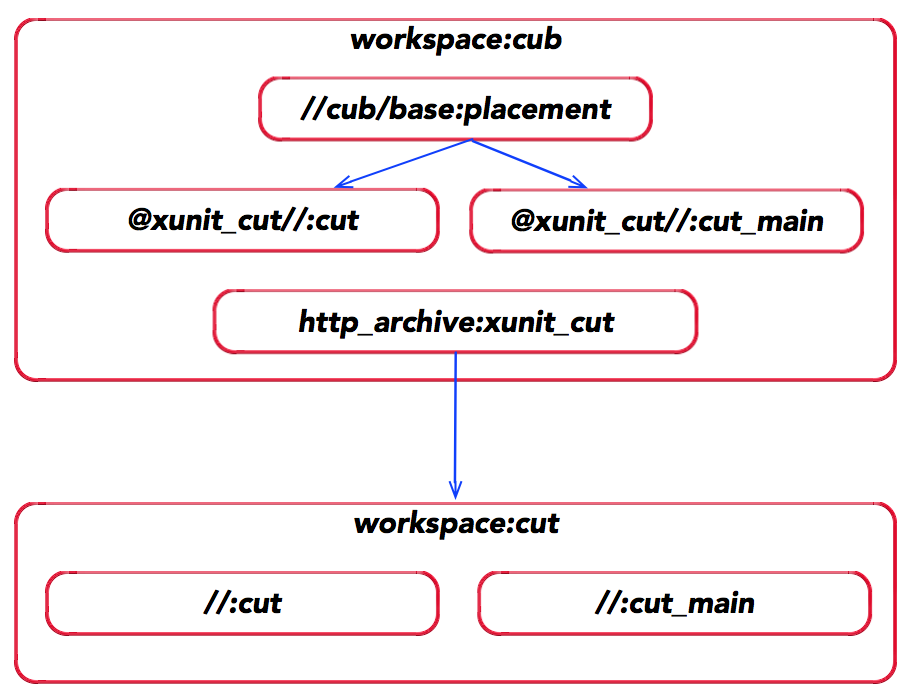
\includegraphics[width=0.8\textwidth]{figures/bazel-concept-cub-deps-cut.png}
\caption{Cub引用外部依赖Cut}
 \label{fig:bazel-concept-cub-deps-cut}
\end{figure}

\subsection{遗留系统}

\ascii{Bazel}推荐的项目组织结构,可能与遗留系统的风格存在迥异。以\ascii{Cut}为例,它原来使用\ascii{CMake}构建,并将\ascii{include, src, test}相互分离,如\refig{bazel-concept-cut}所示。

\begin{figure}[H]
\centering
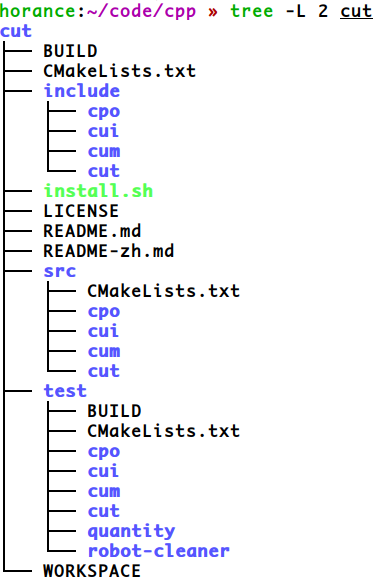
\includegraphics[width=0.6\textwidth]{figures/bazel-concept-cut.png}
\caption{GoogleTest}
 \label{fig:bazel-concept-cut}
\end{figure}

\ascii{Cut}显然违背了\ascii{Bazel}约定的惯例,但它也可以使用\ascii{Bazel}。相对于\ascii{CMake},\ascii{Bazel}的声明式表达,可读性和可维护性相当卓越。

\begin{nodiff}{Cut构建规则}
 \begin{python}
cc_library(
  name = "cut",
  srcs = glob(
      include = [ 
          "src/**/*.cc",
          "src/**/*.cpp"
      ],  
      exclude = [ 
          "src/cut/startup/main.cpp"
      ]      
  ),  
  hdrs = glob([
      "include/**/*.h", "include/**/*.hpp"
  ]), 
  copts = ["-std=c++14"],
  includes = ["include"],
  visibility = ["//visibility:public"],
)

cc_library(
  name = "cut_main",
  srcs = [ 
      "src/cut/startup/main.cpp"
  ],  
  hdrs = [ 
      "include/cut/cut.h",
      "include/cut/startup/StartUp.h",
  ],                                                                                                                        
  copts = ["-std=c++14"],
  includes = ["include"],
  visibility = ["//visibility:public"],
)
 \end{python}
\end{nodiff}

执行如下命令,启动构建\ascii{Cut}。注意,\ascii{BUILD}文件与\ascii{WORKSPACE}在同一目录,标签\ascii{//:cut\_main}的包名为空。

\begin{nodiff}{构建GoogleTest}
 \begin{python}
$ bazel build //:cut_main
 \end{python}
\end{nodiff}

\end{content}


%%%%%%%%%%%%%%%%%%%%%
\appendix

%\part{附录}
%\input{contents/appendix/k8s-cluster.tex}

%%%%%%%%%%%%%%%%%%%%
\backmatter
%\listoffigures
%\myclearpage

%\listoftables
%\myclearpage

\bibliographystyle{alpha}
\renewcommand\bibname{参考文献}
\begin{thebibliography}{20}

\ascii{

\bibitem{agile-principles-1st} Robert C. Martin.
  \newblock \emph{Agile Software Development, Principles, Patterns, and Practices}.

\bibitem{software-craftsman} Robert C. Martin.
  \newblock \emph{The Software Craftsman: Professionalism, Pragmatism, Pride}. 

\bibitem{clean-architecture} Robert C. Martin.
  \newblock \emph{Clean Architecture: A Craftsman's Guide to Software Structure and Design}.  

\bibitem{clean-code} Robert C. Martin. 
  \newblock \emph{Clean Code: A Handbook of Agile Software Craftsmanship}. 

\bibitem{clean-coder} Robert C. Martin.
  \newblock \emph{The Clean Coder: A Code of Conduct for Professional Programmers}. 

\bibitem{tdd-by-example} Kent Beck.
  \newblock \emph{Test Driven Development: By Example}.

\bibitem{xp-explained} Kent Beck.
  \newblock \emph{Extreme Programming Explained: Embrace Change}.

\bibitem{impl-patterns} Kent Beck.
  \newblock \emph{Implementation Patterns}.

\bibitem{refactoring} Martin Fowler, Kent Beck, John Brant, William Opdyke, Don Roberts. 
  \newblock \emph{Refactoring: Improving the Design of Existing Code}. 

\bibitem{dsl} Martin Fowler. 
  \newblock \emph{Domain-Specific Languages}. 

\bibitem{patters-arch} Martin Fowler. 
  \newblock \emph{Patterns of Enterprise Application Architecture}. 

\bibitem{microservices} Sam Newman. 
  \newblock \emph{Building Microservices: Designing Fine-Grained Systems}. 

\bibitem{gof} Erich Gamma, Richard Helm, Ralph Johnson, John Vlissides.
  \newblock \emph{Design Patterns: Elements of Reusable Object-Oriented Software}.

\bibitem{pragmatic-programmer} Andrew Hunt, David Thomas.
  \newblock \emph{The Pragmatic Programmer: From Journeyman to Master}.  

\bibitem{code-complete} Steve McConnell.
  \newblock \emph{Code Complete: A Practical Handbook of Software Construction, 2th Edition}.  

\bibitem{working-with-legacy-code} Michael Feathers.
  \newblock \emph{Working Effectively with Legacy Code}.  

\bibitem{emc} Scott Meyers.
  \newblock \emph{Effective Modern C++: 42 Specific Ways to Improve Your Use of C++11 and C++14}.   

\bibitem{eff-cpp} Scott Meyers.
  \newblock \emph{Effective C++: 55 Specific Ways to Improve Your Programs and Designs}.   

\bibitem{more-eff-cpp} Scott Meyers.
  \newblock \emph{More Effective C++: 35 New Ways to Improve Your Programs and Designs}.   

\bibitem{eff-stl} Scott Meyers.
  \newblock \emph{Effective STL: 50 Specific Ways to Improve Your Use of the Standard Template Library}.   

\bibitem{eff-java} Joshua Bloch.
  \newblock \emph{Effective Java, 3rd Edition}.   

\bibitem{prog-scala} Martin Odersky, Lex Spoon, Bill Venners.
  \newblock \emph{Programming in Scala, 3rd Edition}.   

\bibitem{prog-scala} Martin Odersky, Lex Spoon, Bill Venners.
  \newblock \emph{Programming in Scala, 3rd Edition}.   

\bibitem{tdd-c} James W. Grenning.
  \newblock \emph{Test Driven Development for Embedded C}.   


\bibitem{cpp-template} David Vandevoorde, Nicolai M. Josuttis, Douglas Gregor.
  \newblock \emph{C++ Templates: The Complete Guide}.   

\bibitem{cpp-primer} Stanley B. Lippman, Josée Lajoie, Barbara E. Moo
  \newblock \emph{C++ Primer, 5th Edition}.

\bibitem{programming-bs} Bjarne Stroustrup.
  \newblock \emph{Programming: Principles and Practice Using C++, 2th Edition}.

\bibitem{programming-cpp} Bjarne Stroustrup.
  \newblock \emph{The C++ Programming Language, 4th Edition}.

\bibitem{cpp-concurrency} Anthony Williams.
  \newblock \emph{C++ Concurrency in Action: Practical Multithreading}.

\bibitem{large-cpp-design} John Lakos.
  \newblock \emph{Large-Scale C++ Software Design}.

\bibitem{cpp-coding-std} Herb Sutter, Andrei Alexandrescu.
  \newblock \emph{C++ Coding Standards: 101 Rules, Guidelines, and Best Practices}.

\bibitem{modern-cpp-design} Andrei Alexandrescu.
  \newblock \emph{Modern C++ Design: Generic Programming and Design Patterns Applied}.

\bibitem{ddd} Eric Evans.
  \newblock \emph{Domain-Driven Design: Tackling Complexity in the Heart of Software}.

\bibitem{ddd-prac} Scott Millett, Nick Tune.
  \newblock \emph{Patterns, Principles, and Practices of Domain-Driven Design}.

\bibitem{story-mapping} Jeff Patton, Peter Economy.
  \newblock \emph{User Story Mapping: Discover the Whole Story, Build the Right Product}.


\bibitem{man-month} Frederick P. Brooks Jr.
  \newblock \emph{The Mythical Man-Month: Essays on Software Engineering}.

\bibitem{sicp} Harold Abelson, Gerald Jay Sussman.
  \newblock \emph{Structure and Interpretation of Computer Programs, 2nd Edition}.

\bibitem{c-prog} Brian W. Kernighan, Dennis M. Ritchie.
  \newblock \emph{The C Programming Language, 2nd Edition}.

\bibitem{go-prog} Alan A. A. Donovan, Brian W. Kernighan.
  \newblock \emph{The Go Programming Language}.

\bibitem{pro-git} Scott Chacon, Ben Straub.
  \newblock \emph{Pro Git, 2nd Edition}.

\bibitem{cod} David A. Patterson, John L. Hennessy.
  \newblock \emph{Computer Organization and Design: The Hardware/Software Interface, 5th Edition}.

\bibitem{intro-algo} Thomas H. Cormen, Charles E. Leiserson, Ronald L. Rivest, Clifford Stein.
  \newblock \emph{Introduction to Algorithms, 3rd Edition}.

}

\end{thebibliography}

\endinput

\end{document}
